\begin{pastexam}[label={px:gw3-115-ds-03}]{關務三等資訊處理 115 年 第三題}
（申論；30 分）

\begin{enumerate}[leftmargin=2.6em, labelsep=0.4em]
\item[㈠] 請以下圖的 Graph 為例，分別繪出示意圖，說明程式如何以 adjacency matrix 和 adjacency multilist 二種不同資料
結構儲存此 Graph。（6 分）
\begin{center}
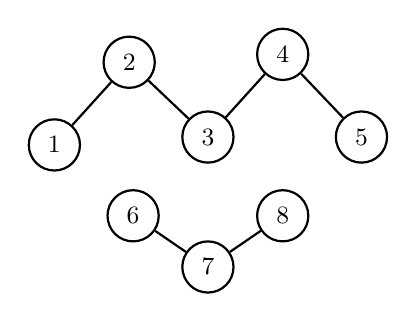
\begin{tikzpicture}[x=1cm,y=1cm,v/.style={circle,draw,thick,inner sep=0pt,minimum size=6.5mm,font=\small}]
\node[v] (1) at (0,0) {1};
\node[v] (2) at (0.95,1.05) {2};
\node[v] (3) at (1.95,0.1) {3};
\node[v] (4) at (2.9,1.15) {4};
\node[v] (5) at (3.9,0.1) {5};
\node[v] (6) at (1.0,-0.9) {6};
\node[v] (7) at (1.95,-1.55) {7};
\node[v] (8) at (2.9,-0.9) {8};
\draw[thick] (1)--(2)--(3)--(4)--(5);
\draw[thick] (6)--(7)--(8);
\end{tikzpicture}
\end{center}
\item[㈡] 若 Graph 有 n 個節點與 e 個邊，請分別說明並以 Big O 寫出 adjacency matrix 和 adjacency multilist 二種不同資料結構
儲存 Graph 時，計算 Graph 中所有節點 Degree 演算法的時間複雜度。（10 分）
\item[㈢] 若 Graph 有 n 個節點與 e 個邊，請分別以 Big O 寫出以 adjacency matrix 和 adjacency multilist 二種不同資料結構儲存
Graph 空間複雜度。比較且說明兩者在空間複雜度的優劣。（14 分）
\end{enumerate}
\end{pastexam}

\begin{pastsoln}
圖是無向圖，$8$ 個節點、$6$ 條邊：(1,\,2)、(2,\,3)、(3,\,4)、(4,\,5)、(6,\,7)、(7,\,8)，分成 $\{1,2,3,4,5\}$ 和 $\{6,7,8\}$ 兩個連通元件。

\textbf{㈠ 鄰接矩陣}（資結書第~21.2~節）：$8 \times 8$ 的陣列，$A[i][j] = 1$ 表示 $i, j$ 之間有邊。 無向圖的矩陣對稱，每條邊
存兩次（$A[i][j]$ 和 $A[j][i]$）。
\begin{center}
\small
\begin{tabular}{c|cccccccc}
 & 1 & 2 & 3 & 4 & 5 & 6 & 7 & 8 \\
\hline
1 & 0 & 1 & 0 & 0 & 0 & 0 & 0 & 0 \\
2 & 1 & 0 & 1 & 0 & 0 & 0 & 0 & 0 \\
3 & 0 & 1 & 0 & 1 & 0 & 0 & 0 & 0 \\
4 & 0 & 0 & 1 & 0 & 1 & 0 & 0 & 0 \\
5 & 0 & 0 & 0 & 1 & 0 & 0 & 0 & 0 \\
6 & 0 & 0 & 0 & 0 & 0 & 0 & 1 & 0 \\
7 & 0 & 0 & 0 & 0 & 0 & 1 & 0 & 1 \\
8 & 0 & 0 & 0 & 0 & 0 & 0 & 1 & 0 \\
\end{tabular}
\end{center}

\textbf{鄰接多重串列}（adjacency multilist）：每條邊只用\textbf{一個}邊節點，由它的兩個端點共用。 邊節點的欄位是
\[
\boxed{\ \mathit{mark}\ \big|\ v_1\ \big|\ v_2\ \big|\ \mathit{link}_1\ \big|\ \mathit{link}_2\ }
\]
$\mathit{mark}$ 記錄這條邊走訪過沒有；$\mathit{link}_1$ 指向下一個「含 $v_1$」的邊節點，$\mathit{link}_2$ 指向下一個「含 $v_2$」
的邊節點。 另有一個頂點陣列 $\mathit{head}[1..8]$，$\mathit{head}[v]$ 指向第一個含 $v$ 的邊節點。 從 $\mathit{head}[v]$ 出發，
每到一個邊節點，看 $v$ 是 $v_1$ 還是 $v_2$，就沿 $\mathit{link}_1$ 或 $\mathit{link}_2$ 走，可以走遍 $v$ 的所有邊。

本圖把邊編為 $E_1$ 到 $E_6$：
\begin{center}
\small
\begin{tabular}{c@{\qquad}c}
\begin{tabular}{c|c}
\toprule
頂點 & $\mathit{head}$ \\
\midrule
1 & $E_1$ \\
2 & $E_1$ \\
3 & $E_2$ \\
4 & $E_3$ \\
5 & $E_4$ \\
6 & $E_5$ \\
7 & $E_5$ \\
8 & $E_6$ \\
\bottomrule
\end{tabular}
&
\begin{tabular}{c|ccccc}
\toprule
邊節點 & $\mathit{mark}$ & $v_1$ & $v_2$ & $\mathit{link}_1$ & $\mathit{link}_2$ \\
\midrule
$E_1$ & 0 & 1 & 2 & \NIL & $E_2$ \\
$E_2$ & 0 & 2 & 3 & \NIL & $E_3$ \\
$E_3$ & 0 & 3 & 4 & \NIL & $E_4$ \\
$E_4$ & 0 & 4 & 5 & \NIL & \NIL \\
$E_5$ & 0 & 6 & 7 & \NIL & $E_6$ \\
$E_6$ & 0 & 7 & 8 & \NIL & \NIL \\
\bottomrule
\end{tabular}
\end{tabular}
\end{center}
讀法：頂點 $3$ 的邊從 $\mathit{head}[3] = E_2$ 開始；$3$ 是 $E_2$ 的 $v_2$，沿 $\mathit{link}_2$ 到 $E_3$；$3$ 是 $E_3$ 的
$v_1$，沿 $\mathit{link}_1$ 得 \NIL，結束。 所以頂點 $3$ 的邊是 $E_2 = (2,3)$、$E_3 = (3,4)$。 頂點 $2$：$E_1$（$v_2$）$\to E_2$
（$v_1$）$\to$ \NIL。 每個邊節點被兩個頂點的串列共用，例如 $E_2$ 同時在頂點 $2$ 和頂點 $3$ 的串列裡。

\textbf{㈡ 計算所有節點的 degree}。
\begin{itemize}
\item \textbf{鄰接矩陣}：頂點 $i$ 的 degree 是第 $i$ 列 $1$ 的個數，每列要看 $n$ 格，$n$ 列共 $n^2$ 格，時間 $O(n^2)$。
不論邊多少都一樣，因為沒有邊的 $0$ 也要看過。
\item \textbf{鄰接多重串列}：對每個頂點 $v$，從 $\mathit{head}[v]$ 沿串列數邊節點的個數。 每個邊節點恰好被它的兩個端點
各走到一次，所以總共走 $2e$ 步，加上 $n$ 個串列頭，時間 $O(n + e)$。 更直接的做法：把 $\mathit{deg}[1..n]$ 清成 $0$，
掃過每個邊節點一次，把 $\mathit{deg}[v_1]$、$\mathit{deg}[v_2]$ 各加 $1$，也是 $O(n + e)$。
\end{itemize}
本圖：degree 依序是 $1, 2, 2, 2, 1, 1, 2, 1$，總和 $12 = 2e$。

\textbf{㈢ 空間複雜度}。
\begin{itemize}
\item \textbf{鄰接矩陣}：$n^2$ 格，$O(n^2)$。 （利用對稱只存上三角也要 $n(n-1)/2$ 格，仍是 $O(n^2)$。）
\item \textbf{鄰接多重串列}：$n$ 個頂點的串列頭加上 $e$ 個邊節點，每個邊節點固定 $5$ 個欄位，$O(n + e)$。
\end{itemize}
比較：
\begin{itemize}
\item \textbf{邊少（稀疏圖，$e$ 遠小於 $n^2$）時多重串列省很多}。 矩陣不管有沒有邊都佔 $n^2$ 格，例如 $n = 10000$ 而每個頂點
只有幾條邊，矩陣要一億格，多重串列只要數萬個欄位。 本題 $n = 8$、$e = 6$：矩陣 $64$ 格；多重串列 $8$ 個頭指標加
$6 \times 5 = 30$ 個欄位。
\item \textbf{邊多（稠密圖，$e$ 接近 $n(n-1)/2$）時矩陣較好}。 兩者都是 $\Theta(n^2)$，但矩陣每格只要 $1$ 個位元，多重
串列每條邊要兩個頂點編號和兩個指標，常數大得多。
\item 和一般的鄰接串列比，多重串列每條邊只用一個節點（一般鄰接串列每條邊在兩端各存一個，共 $2e$ 個），但每個節點的
欄位比較多，總空間同樣是 $O(n + e)$、相差不大。 它的好處在於同一條邊只有一份，$\mathit{mark}$ 欄位讓「每條邊只處理一次」的
演算法（例如走訪所有邊）很方便。
\end{itemize}
\end{pastsoln}
